The results obtianed with the simulation described in section \ref{subsec:SourceShapeSimulation} are shown and discussed in this section. The objective of these simulations is to decide which is the radial thick of the simulated tritium source that optimize the simulations. 

First, the energy of the simulated tritium events are verified. For this task, the energy distribution of the simulated tritium electrons is obtained and shown in figure \ref{subfig:EnergyDistributionTritiumSource}, which is compared with that obtained in the reference \cite{TritiumEmissionSpectrum}. As can be checked, there is a good agreement between both.

\begin{figure}[h]
 \centering
  \subfloat[Energy distribution of tritium decays simulated]{
   \label{subfig:EnergyDistributionTritiumSource}
    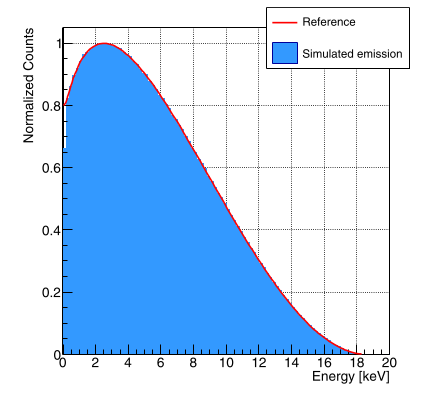
\includegraphics[width=0.5\textwidth]{8SimulationsResults/81TRITIUMDesign/TritiumSourceEnergyDistribution.png}}
   %\newline
  \subfloat[]{
   \label{subfig:EnergySpectrumEventsDetectedandNonDetected}
    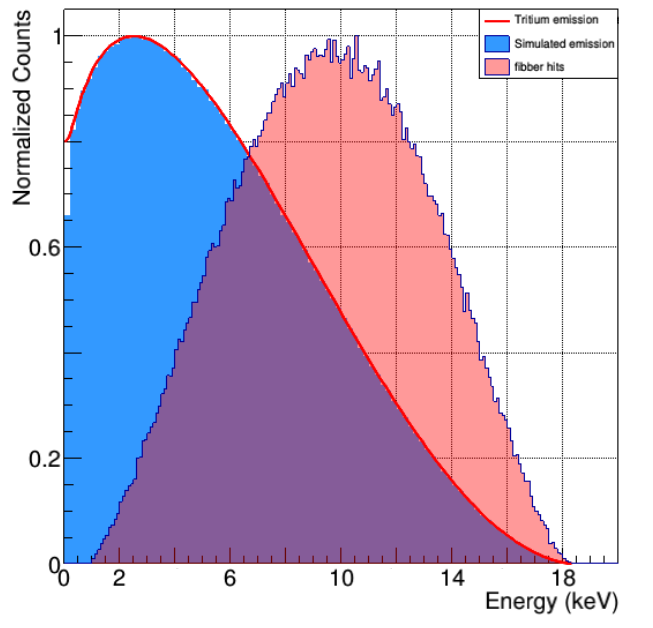
\includegraphics[width=0.5\textwidth]{8SimulationsResults/81TRITIUMDesign/Source_Spectrum_yes_and_non_detected_events.png}}
 \caption{ Energy distribution of a) simulated tritium decays b) Initial energy of tritium decays that reach the scintillating fibers (red histogram) compared the all simulated tritium events (blue histogram).}
 \label{fig:TritiumSourceOptimization}
\end{figure}

In addition, an energy spectrum of the initial energy of the detected tritium electrons are shown in Figure \ref{subfig:EnergySpectrumEventsDetectedandNonDetected}, red histogram, which is compared to the energy distribution of all simulated tritium events. As can be seen, the red histogram are centred at $10~\keV$ since the lower energy tritium events do not reach the scintillating fibers. This occurs mainly because they are absorbed at a very short distance in the water volume or they don't have enough energy to overcome the water-fiber interface.

Figure \ref{subfig:TransversalCutTritiumSource} shows a transversal cut of the $2~\mm$ scintillating fiber, yellow, the simulated tritium source $0.5~\mm$ thick around the fiber, green, and the tritium decays, red dots, the electrons of which has been absorbed in the fiber.

\begin{figure}[h]
 \centering
  \subfloat[]{
   \label{subfig:TransversalCutTritiumSource}
    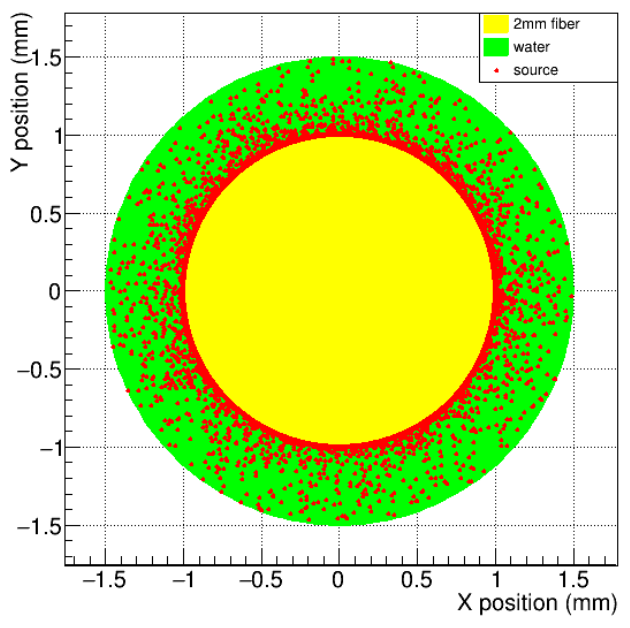
\includegraphics[width=0.5\textwidth]{8SimulationsResults/81TRITIUMDesign/Source_Ring.png}}
   %\newline
  \subfloat[]{
   \label{subfig:DistanceDistributionTritiumSourceFiber}
    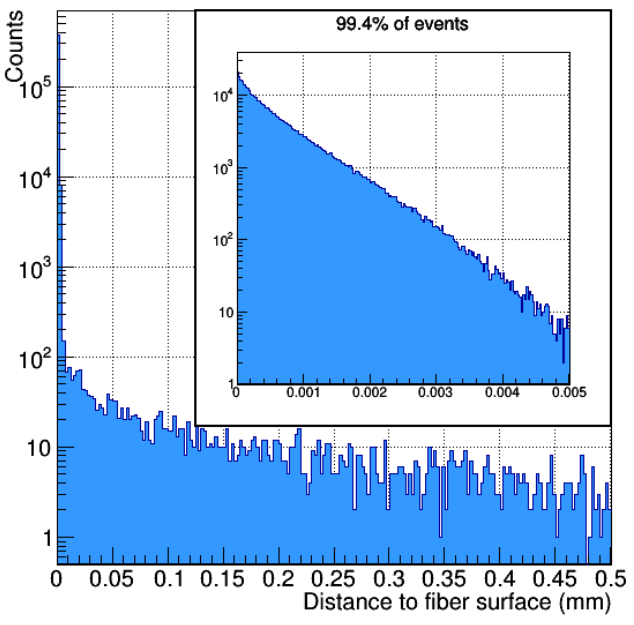
\includegraphics[width=0.5\textwidth]{8SimulationsResults/81TRITIUMDesign/SourceDistance.png}}
 \caption{a)Transversal cut of simulated scintillating fiber (yellow) and tritium source (green) with various tritium decays (red dots) b) Distribution of the radial distance between the position where the tritium decay takes place and the surface of the scintillating fiber.}
 \label{fig:TritiumSourceSimulated}
\end{figure}	

As can be seen, most of the tritium decays that are detected occur in close proximity to the scintillating fiber. A histogram of the radial distance between the position where tritium decays take place and the surface of the scintillating fiber are shown in figure \ref{subfig:DistanceDistributionTritiumSourceFiber}. It can be verified again that most of the detected tritium decays has happened in positions very close to the fiber. A zoom is applied in the inset box where it can be appreciate that the $99.4\%$ of the detected events are produced at least of $5~\mu\meter$, which is the mean free path of tritium electrons. Therefore, the thick of the simulated tritium source chosen to optimize the simulation are $5~\mu\meter$. 

